\subsubsection{\bf Introduction}
RayleighMonitor is a tool for calculated a quantile value of normalized spectrum of $x(t)$.
The deviation of the calculated quantiles from the expected one in Gaussian noise case
shows deviation of the detector noise from Gaussian distribution.

Normalized spectrogram, $w(t, f)$, of input signal, $x(t)$, is calculated
\begin{align*}
  w(t_i,~f_j) = \frac{ |~{\rm STFT}[x(t)]~| }{S_{\rm 0}(f)},
\end{align*}
where $1\leq i\leq N$, ~$1\leq j\leq M$ and $S_{\rm 0}(f)$ is a normalization factor.
Normalization factor can be estimated
\begin{align*}
  S_{\rm 0}(f) = |~{\rm FFT}[x(t)]~|.
\end{align*}
P-quantile value of input signal is calculated from normalized spectrogram as the function of time and frequency,
$Q(P;~f_l)$ where $1\leq l\leq M/m$, $m(l-1)-1\leq j\leq ml$
and $m = {\rm d}f/{\rm d}f_{\rm fft} = {\rm d}f~{\rm d}t_{\rm fft}$

\subsubsection{{\bf Function:} rayleighMonWaveData}
{\tt ~ rayleighMonWaveData p secfft df x0 xt\\}

This function compute p-quantile value, $Q(p;~f)$, of the input signal, $x(t)$, as the function of frequency, $f$.
The arguments are:
\begin{itemize}
\item {\tt p}: Input. The list of dimensionless p-values ($0 \leq p \leq 1$).
\item {\tt secfft}: Input. The data length for short time Fourier transform in seconds.
\item {\tt df}: Input. The frequency resolution of $Q(p;~f)$ in Hertz
\item {\tt x0}: Input. The time series signal for estimating averaged spectrum
\item {\tt xt}: Input. The time series for calculating quantile value $Q(p;~f)$
\item {\tt q}: Output. The quantile value of input signal $Q(p;~f)$.
\end{itemize}

\subsubsection{{\bf Example:} rayleighMon}
This program calculates the $Q(p;~f)$ of the input signal.\\

{\noindent \bf Typical usage:} {\tt rayleighMon param.conf file.lst}
{\footnotesize
\begin{verbatim}
  import Data.Maybe (catMaybes)
  import System.Environment (getArgs)

  import HasKAL.DetectorUtils.Detector (Detector(..))
  import HasKAL.FrameUtils.Function (readFrameWaveData')
  import HasKAL.Misc.ConfFile (readFileList, readConfFile)
  import HasKAL.MonitorUtils.RayleighMon.RayleighMon (rayleighMonWaveData)
  import HasKAL.PlotUtils.HROOT.PlotGraph
  import HasKAL.WaveUtils.Data (WaveData(..))
  import HasKAL.WaveUtils.Function (catWaveData)

  main = do
    {-- arg check --}
    args <- getArgs
    (conf, lst) <- case length args of
                    2 -> return (args!!0, args!!1)
                    _ -> error Usage: rayleighMon conffile filelist"

    {-- read param --}
    filelist <- readFileList lst
    ([ch, dtfft, df], [qs]) <- readConfFile conf ["channel", "dtfft", "df"] ["quantile"]

    {-- read data --}
    mbWd <- mapM (readFrameWaveData' KAGRA ch) filelist
    let wd = case catMaybes mbWd of
              [] -> error "Can't find file."
              xs -> catWaveData xs

    {-- main --}
    let result = rayleighMonWaveData (map read qs) (read dtfft) (read df) wd wd
        lineType = concat $ replicate (length qs) [LinePoint, Line]
        colors = concatMap (replicate 2) [RED, BLUE, PINK, GREEN, CYAN, YELLOW, BLACK]
        title = ch ++ ": " ++ (show . fst . startGPSTime $ wd) ++ " ~ " ++ (show . fst . stopGPSTime $ wd)
    oPlotV Linear lineType 1 colors ("frequency [Hz]", "normalized noise Lv.") 0.05
    title "X11" ((0,0),(0,0)) $ concatMap (\(x,y) -> [x,y]) result

\end{verbatim}
}


{\noindent \bf Param file format:} {\tt param.conf}
{\footnotesize
\begin{verbatim}
  channel: X1:HOGE-XX  # channel name
  quantile: 0.5 0.95   # list of dimensionless p-value
  dtfft: 1             # data length for STFT in seconds
  df: 16               # frequency resolution of Q(p;~f) in Hertz

\end{verbatim}
}

{\noindent \bf List file format:} {\tt file.lst}
{\footnotesize
\begin{verbatim}
  /path/to/framefile/a.gwf
  /path/to/framefile/b.gwf

\end{verbatim}
}

\begin{figure}[t]
 \begin{center}
    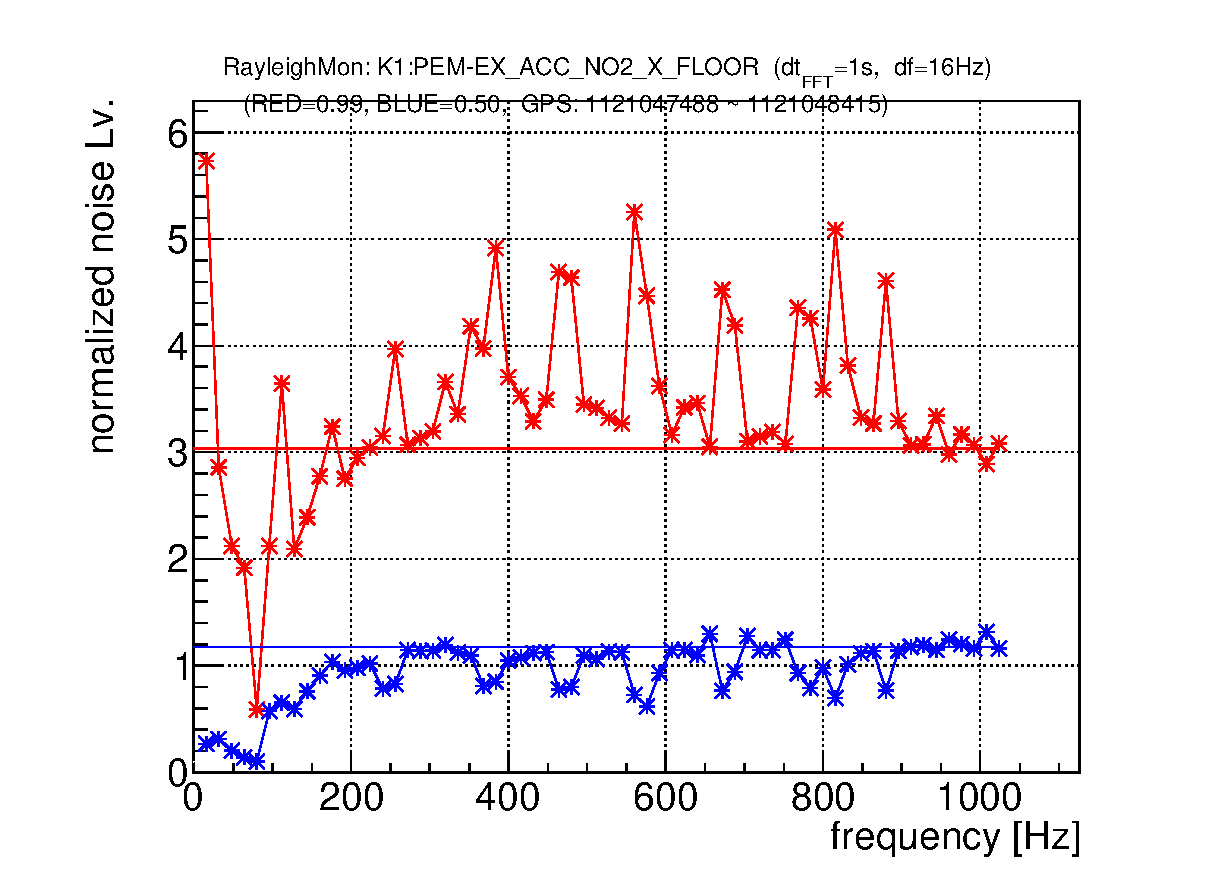
\includegraphics[width=0.9\hsize]{fig/RayleighMon/sample1.eps}
    \caption{sample plot of rayleighMonitor}
 \end{center}
\end{figure}

{\noindent \small contact person: Takahiro Yamamoto (\tt yamamoto@yukimura.hep.osaka-cu.ac.jp)}

